\chapter{Frequency analysis} \label{ch9}
In this chapter the results from the recordings described in appendix \ref{recordings} will undergo frequency analyses. This will detect the frequency compositions of the music and noise signals, which will aid the design of a filter designated to filter out noise. The frequency analyses is furthermore necessary for the creation of spectrograms illustrating the frequency compositions of the signals in time. \\ \\
This project includes an implementation of the Cooley-Tukey FFT algorithm in Python but the results of this algorithm are identical to the FFT included in the Numpy-package in Python, which is much faster than the implementation described in algorithm \ref{FFTalg}. The FFT from Numpy will therefore be used for the frequency analyses in this chapter.

\section{Frequency analysis of music}
In this section the recordings of music will undergo frequency analysis, and the goal is to be able to express which frequencies the tones played in the recordings are generally found at. It is expected that both the significant tone and its corresponding harmonics will appear in the frequency spectrum.
   
\subsection{Single tone} \label{sec:single}
Firstly, the tuning of guitar is checked for consistency. The low and high E strings on the guitar should vibrate and emit sounds frequencies of 82.41 Hz and 329.63 Hz, respectively, as seen in table \ref{fig:guitar_frequencies}. Figures \ref{fig:single_low} and \ref{fig:single_high} show the frequency spectra for the recordings of the two tones.
\begin{figure}[H]
\centering
\begin{subfigure}{0.49\textwidth}
\centering
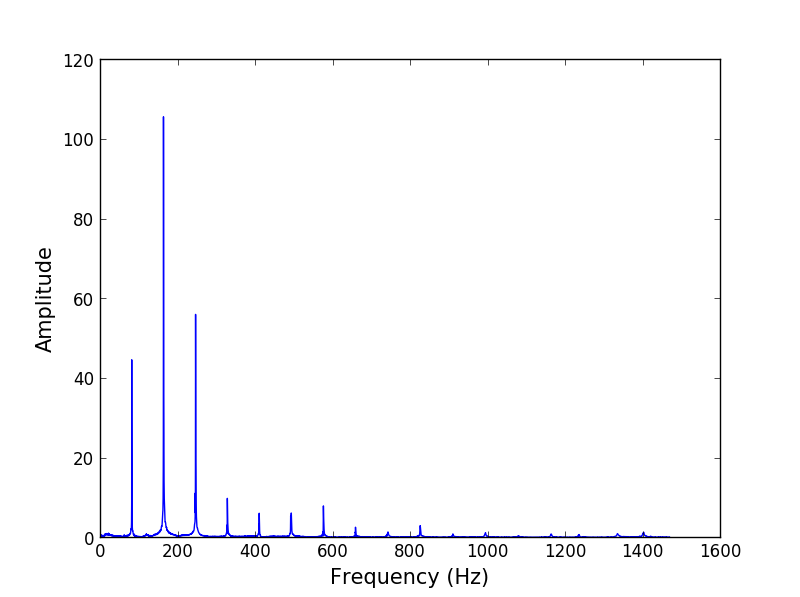
\includegraphics[width=\textwidth]{figures/freqanal/single_low.png}
\caption{Low E string}
\label{fig:single_low}
\end{subfigure}
\begin{subfigure}{0.49\textwidth}
\centering
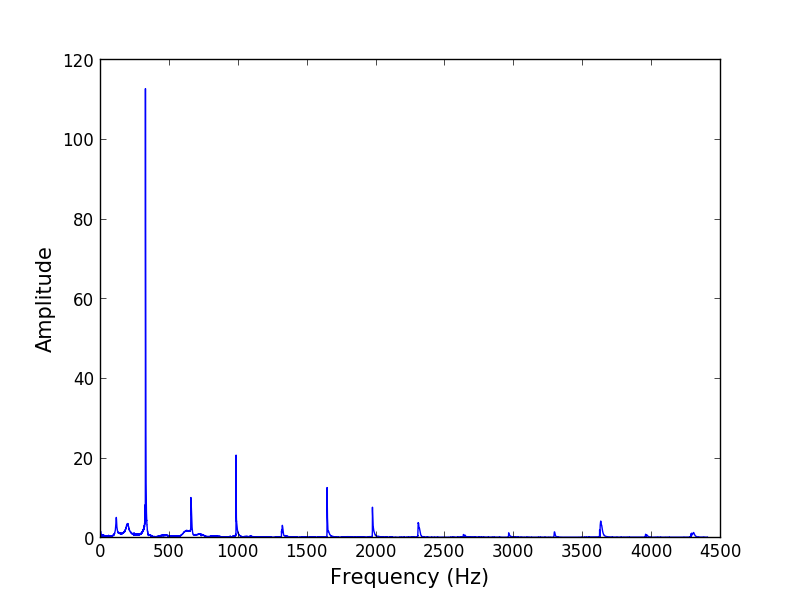
\includegraphics[width=\textwidth]{figures/freqanal/single_high.png}
\caption{High E string}
\label{fig:single_high}
\end{subfigure}
\caption{Frequency spectra of low and high E strings on a guitar. The harmonics are clearly visible.}
\label{fig:single}
\end{figure}
\martin{Frederik retter de her grumme figurer.}

With a peak detection algorithm implemented in Python the most significant frequencies in the two recordings are registered to be 163.82 Hz and 329.83 Hz for the low and high E's, respectively. As $163.82$ Hz $\approx 2\cdot82.41$ Hz this is regarded as a harmonic of the low E. The harmonics are moreover observable in the figures as reduced peaks at integer multiples of the fundamental frequencies of the tones. It is furthermore seen from the figures, that the energy in the signals is mainly located at frequencies above 75 Hz and below 1000 Hz for the low E and above 100 Hz and below 2000 Hz for the high E.\\ 

\subsection{Chord}
Figures \ref{fig:chord_low} and \ref{fig:chord_high} show the frequency spectra of the recordings of low and high E chords, respectively.
\begin{figure}[H]
\centering
\begin{subfigure}{0.49\textwidth}
\centering
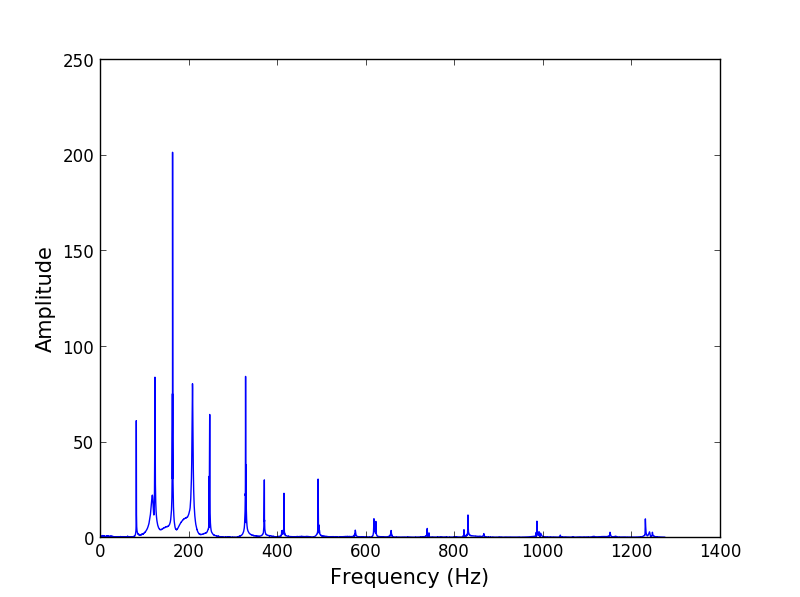
\includegraphics[width=0.9\textwidth]{figures/freqanal/chord_low.png}
\caption{Low E chord.}
\label{fig:chord_low}
\end{subfigure}
\begin{subfigure}{0.49\textwidth}
\centering
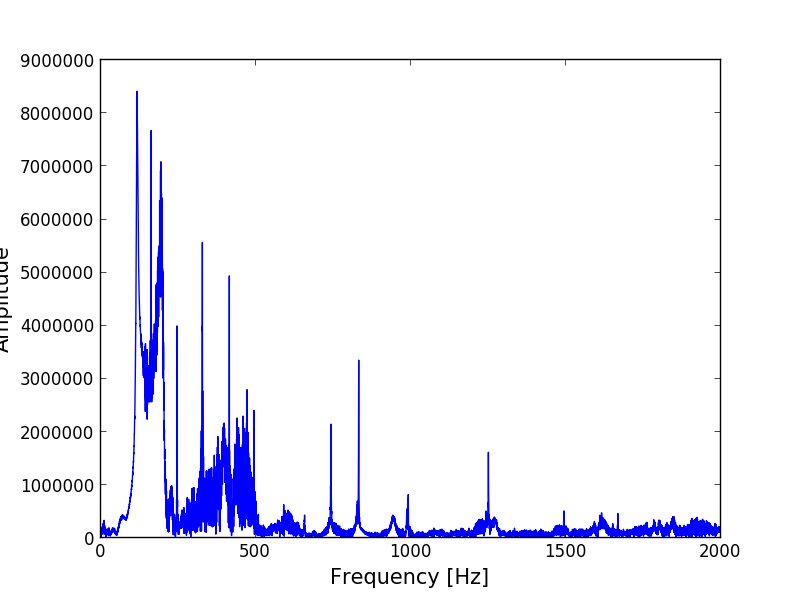
\includegraphics[width = \textwidth]{figures/freqanal/chord_high.png}
\caption{High E chord.}
\label{fig:chord_high}
\end{subfigure}
\caption{Frequency spectra of low and high E chords played on a guitar.}
\label{fig:chord}
\end{figure}

The most significant frequencies in figure \ref{fig:chord_low} is 163.86 Hz and 119.27 Hz in figure \ref{fig:chord_high}. Once again it is assumed that the higher frequency of the low pitch E is due to harmonics. The second frequency does furthermore not correspond to a specific note - this is assumed to be because of the composition of chords being of multiple tones. The majority of the energy in the signals is located above 80 Hz and below 1000 Hz.
\subsection{Scale}
Figure \ref{fig:scale_fast} shows the frequency spectrum of playing a octatonic scale.
\begin{figure}[H]
\centering
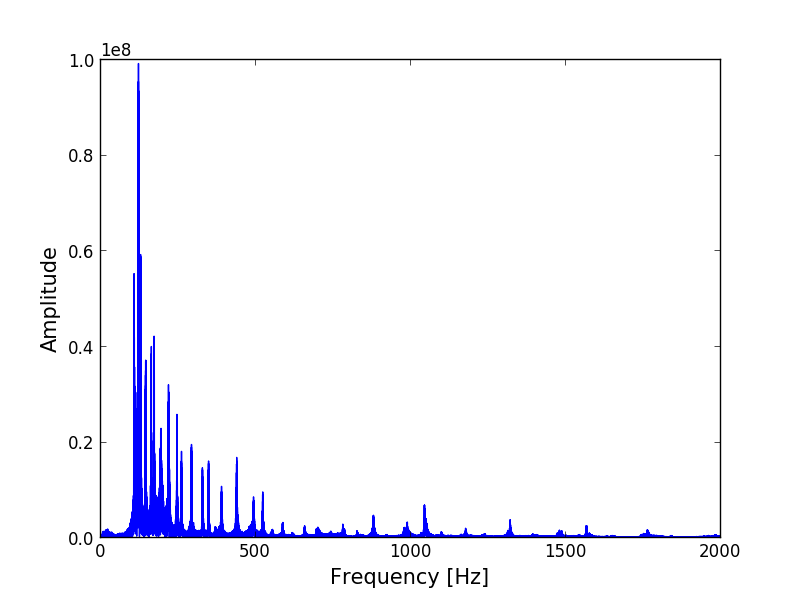
\includegraphics[width=0.7\textwidth]{figures/freqanal/scale_fast.png}
\caption{Frequency spectrum of an octatonic scale played quickly.}
\label{fig:scale_fast}
\end{figure}
The majority of the energy in the signal is as seen located above 100 Hz and below 600 Hz.

\subsection{Melody with single notes}
Figures \ref{fig:melody_single} show the frequency spectrum for a melody consisting only of single tones played slowly.
\begin{figure}[H]
\centering
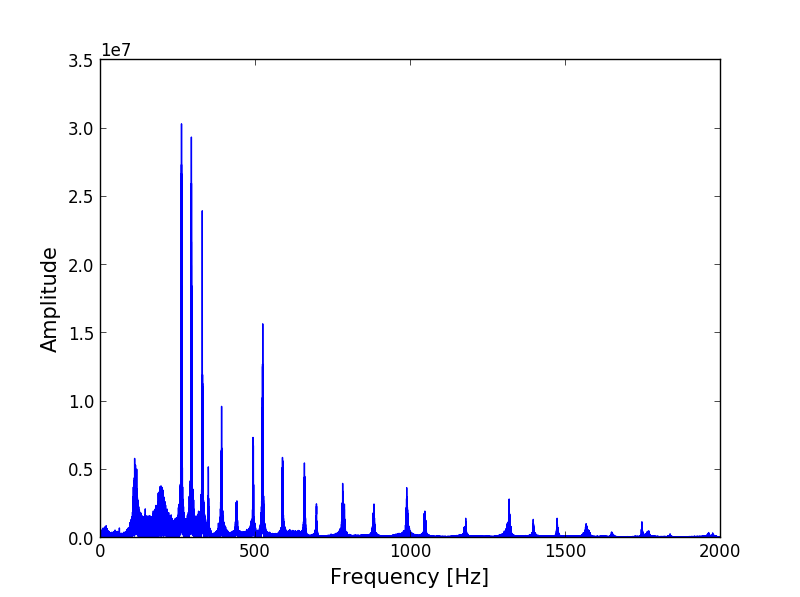
\includegraphics[width=0.7\textwidth]{figures/freqanal/melody_single.png}
\caption{Frequency spectrum of Itsy Bitsy Spider played on a guitar with only single strings plucked.}
\label{fig:melody_single}
\end{figure}
The majority of energy in the signal is located above 100 Hz and below 2000 Hz.

\section{Frequency analysis of noise}
In this section the recordings of noise will undergo frequency analysis, and the goal is to be able to express which frequencies the recorded noise is generally found at.
\subsection{Folding paper and clapping}
Figure \ref{fig:clapping} and \ref{fig:folding} show the frequency spectrum of clapping at equidistant intervals in time and folding a piece of paper, respectively.
\begin{figure}[H]
\centering
\begin{subfigure}{0.49\textwidth}
\centering
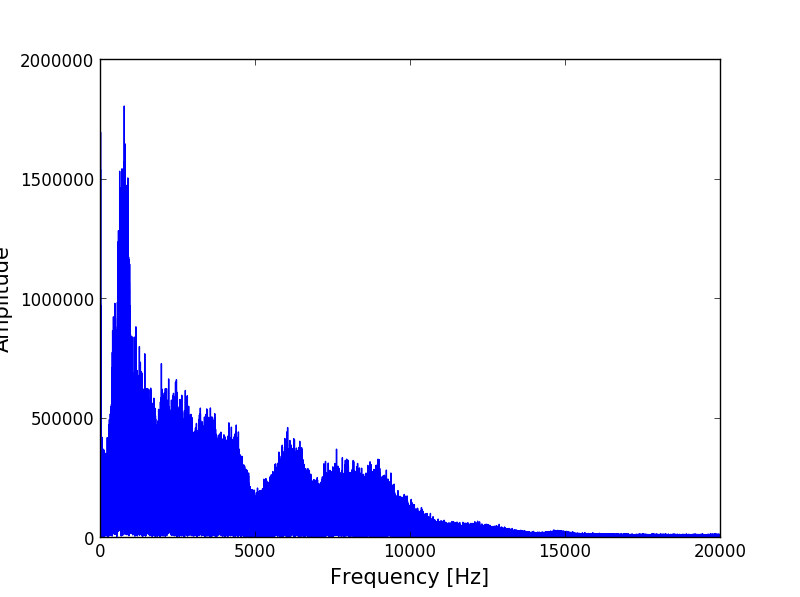
\includegraphics[width=\textwidth]{figures/freqanal/clapping.png}
\caption{Clapping}
\label{fig:clapping}
\end{subfigure}
\begin{subfigure}{0.49\textwidth}
\centering
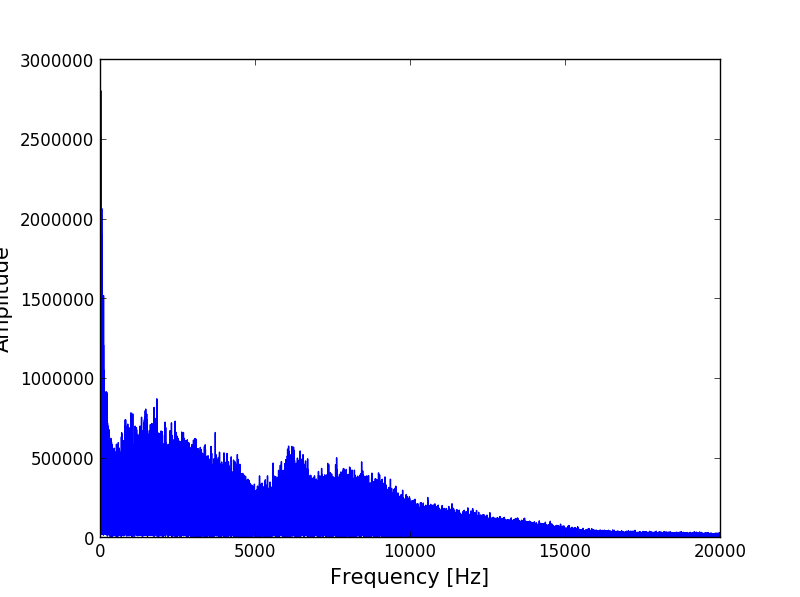
\includegraphics[width=\textwidth]{figures/freqanal/folding.png}
\caption{Folding a piece of paper}
\label{fig:folding}
\end{subfigure}
\caption{Frequency spectra of different noises.}
\end{figure}
The majority of the energy in both noises is located between 0 and 15000 Hz.
%\subsection{Singing and talking}
%Figures \ref{fig:talk} and \ref{fig:song} show the frequency spectrum of recorded talking and singing respectively.
%\begin{figure}[H]
%\centering
%\begin{subfigure}{0.49\textwidth}
%\centering
%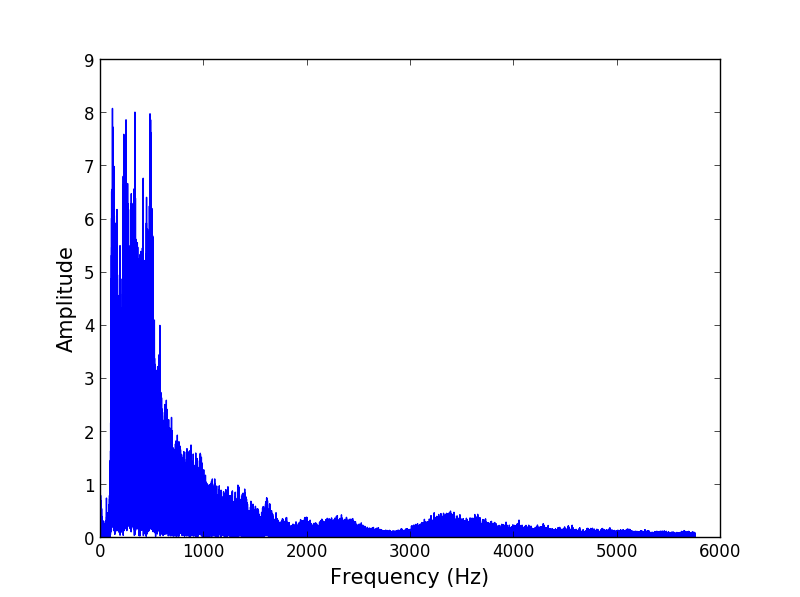
\includegraphics[width=\textwidth]{figures/freqanal/talk.png}
%\caption{Person talking}
%\label{fig:talk}
%\end{subfigure}
%\begin{subfigure}{0.49\textwidth}
%\centering
%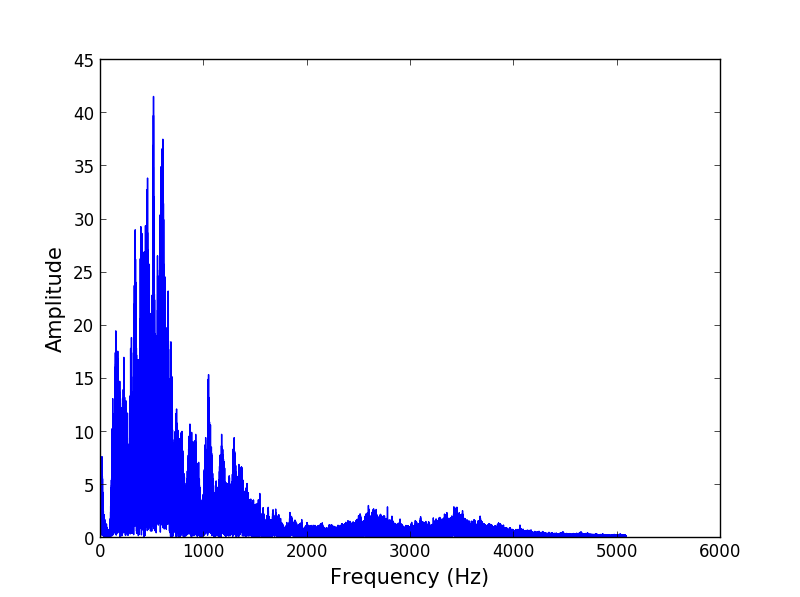
\includegraphics[width=\textwidth]{figures/freqanal/song.png}
%\caption{Person singing}
%\label{fig:song}
%\end{subfigure}
%\caption{Frequency spectra of a person talking and signing.}
%\end{figure}
%The majority of the energy is located between 100 and 5000 Hz for talking and 0 and 5000 Hz for singing.
\subsection{Ambient noise}
Figure \ref{fig:ambient} shows the frequency spectrum of the ambient noise recorded in a parking lot at the campus of AAU.
\begin{figure}[H]
\centering
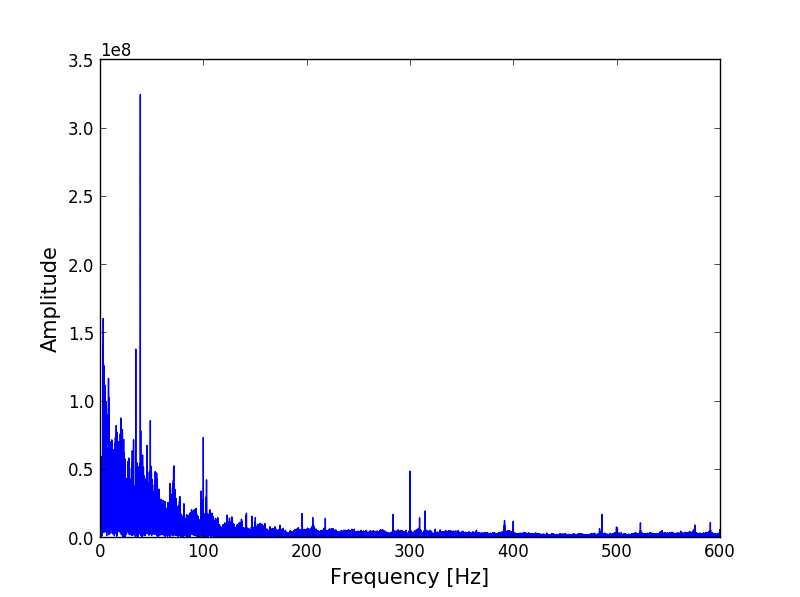
\includegraphics[width=0.7\textwidth]{figures/freqanal/ambient.png}
\caption{Frequency spectrum for ambient sound.}
\label{fig:ambient}
\end{figure}
The majority of the energy in the signal is located between 0 and 600 Hz.













\section{Filter design}
In this section, the frequency analysis of the music and noise in the former sections form the basis for the design of the filter, whose aim is to filter out the noise. The noise is both low- and high-frequency, whereas the frequency of the music lies in the middle, which means that the filter should be a bandpass filter. From the discussion of different filters and designs of these in chapter \ref{ch8} the implemented filter is furthermore chosen to be a FIR filter since this type of filter is guaranteed to have linear phase, which preserves the wave form of the original signal, which of course is important in this project. Furthermore, FIR filters are rather easy to design. On the downside, a FIR filter uses many computations, which is problematic if the filter is supposed to run in real time - that is, while the music is being played. However, in this project the music is first recorded and then analysed, which means that the computations are not a big factor. For an actual system working in real time the amount of computations plays a bigger factor, and such a system could be considered to use an IIR filter but the linear phase from the FIR filter is weighted as more important in this particular project.